\documentclass[]{article}
\usepackage[T1]{fontenc}
\usepackage{lmodern}
\usepackage{amssymb,amsmath}
\usepackage{fullpage}
\usepackage{ifxetex,ifluatex}
\usepackage{fixltx2e} % provides \textsubscript
% use microtype if available
\IfFileExists{microtype.sty}{\usepackage{microtype}}{}
\ifnum 0\ifxetex 1\fi\ifluatex 1\fi=0 % if pdftex
  \usepackage[utf8]{inputenc}
\else % if luatex or xelatex
  \usepackage{fontspec}
  \ifxetex
    \usepackage{xltxtra,xunicode}
  \fi
  \defaultfontfeatures{Mapping=tex-text,Scale=MatchLowercase}
  \newcommand{\euro}{€}
\fi
% Redefine labelwidth for lists; otherwise, the enumerate package will cause
% markers to extend beyond the left margin.
\makeatletter\AtBeginDocument{%
  \renewcommand{\@listi}
    {\setlength{\labelwidth}{4em}}
}\makeatother
\usepackage{enumerate}
\usepackage{graphicx}
% We will generate all images so they have a width \maxwidth. This means
% that they will get their normal width if they fit onto the page, but
% are scaled down if they would overflow the margins.
\makeatletter
\def\maxwidth{\ifdim\Gin@nat@width>\linewidth\linewidth
\else\Gin@nat@width\fi}
\makeatother
\let\Oldincludegraphics\includegraphics
\renewcommand{\includegraphics}[1]{\Oldincludegraphics[width=\maxwidth]{#1}}
\ifxetex
  \usepackage[setpagesize=false, % page size defined by xetex
              unicode=false, % unicode breaks when used with xetex
              xetex]{hyperref}
\else
  \usepackage[unicode=true]{hyperref}
\fi
\hypersetup{breaklinks=true,
            bookmarks=true,
            pdfauthor={Harshal Pandya and Brian Martin},
            pdftitle={CS677: Lab 1},
            colorlinks=true,
            urlcolor=blue,
            linkcolor=magenta,
            pdfborder={0 0 0}}
\setlength{\parindent}{0pt}
\setlength{\parskip}{6pt plus 2pt minus 1pt}
\setlength{\emergencystretch}{3em}  % prevent overfull lines
\setcounter{secnumdepth}{0}

\title{CS677: Lab 1}
\author{Harshal Pandya and Brian Martin}
\date{}

\begin{document}
\maketitle

Our system implements the provided spec: a pig2pig network in which pigs
collaborate to avoid impact with an adversarial bird.

\subsection{Game Map}

The game map is single-dimensional with pigs and columns placed
randomly. It is assumed that the bird is always launched from the left
(as in the original Angry Birds). The ratio of columns to pigs is at
most one.

\subsection{Assumed Physics}

We assume that certain behaviors for each element type:

\begin{itemize}
\item
  \textbf{Pig}: An impacted pig will fall to the right (as the bird
  always approaches from the left). If a pig falls onto another pig both
  are considered impacted, but the second pig does not change position
  on impact. If a pig is impacted while having a column to the right,
  then that column will also fall to the right, affecting any pig which
  may find itself in that position.
\item
  \textbf{Column}: If a column is impacted directly, then it falls to
  the right, only affecting any pig or column to its immediate right.
\end{itemize}

\subsection{Game Engine}

In our system the \emph{game engine} has several roles:

\begin{enumerate}[1.]
\item
  Map generation
\item
  Pig network topology generation
\item
  Sending round-initiating trajectory message to the nearest pig.
\item
  Ends the round.
\end{enumerate}

\subsection{Pigs as Actors}

Each pig functions as an actor which can recieve and act on several
message types, derived from the original specification:

\begin{itemize}
\item
  \texttt{Trajectory(position: Int)} notifies the nearest pig about the
  birds trajectory.
\item
  \texttt{BirdApproaching(targetPosition: Int, hopCount: Int)} used by
  the nearest bird to initiate a round of notifications the pig being
  hit.
\item
  \texttt{TakeShelter(position: Int, hopCount: Int)} used by the pig
  directly hit to notify other pigs to take shelter if they are a part
  of the collateral damage.
\item
  \texttt{Status(pigId: Int)} used to query each pig about its safety.
\item
  \texttt{EndGame} used by the Master to end the round.
\end{itemize}

\subsection{Launching a bird}

A bird launch is described by the time the master picks a random target
and notifies the nearest pig about the trajectory. It then picks a
random time to target before sending an end game message thus signaling
that the bird has landed.

\section{Description of ``how it works''}

We use the Actor framework to enable communication between machines. The
Actor model is a mathematical model of concurrent computation that
treats ``actors'' as the universal primitives of concurrent digital
computation: in response to a message that it receives, an actor can
make local decisions, create more actors, send more messages, and
determine how to respond to the next message received. Each pig is an
Actor in our system which is essentially a stub on a remote jvm. The
actors exchange messages among themselves and take actions in response
according to the game logic. On receiving the BirdApproaching message,
the actor checks if it is directly impacted by the approaching bird, if
so it tries to move. If it can't move since it's blocked, it sends out a
TakeShelter message to the other actors. On receiving the TakeShelter
message the actors check to see if they are close to a pig or column
being hit and move if required and is possible. After the master sends
the EndGame message signaling the bird landing, the pigs update their
states to know whether they were hit or not using the messages still
being flooded. On receiving the status query, each pig responds with a
wasHit message.

\section{Design Decisions / Trade-offs}

The pigs form a bidirectional ring topology and messages are passed both
ways. The pigs don't maintain any state apart from their current
locations in the world. If they are being affected they change locations
and all the other messages get ignored once they are in a safe spot.

We use hopcounts to limit the the lifetime of messages propagating
through the system. Without a hopcount messages would flow from pig to
pig forever.

We do not maintain a shared map data structure and hence the map is not
updated when the pigs move. This however saves the effort of maintaing a
synchronous thread-safe data structure that lives on the master and adds
extra messages to the system.

\section{Possible Improvements}

A more complex topology instead of a simple bidirectional ring would be
a good experiment. In terms of the game logic, we could use a 2
dimensional world. Also we could make pigs move make space for pigs
being affected and have the effect of hits cascade beyond 2 positions.

\section{How to run the program}

We require \texttt{maven}, the Java dependency management tool, to pull
in all dependencies and generate a jar file of compiled code.

We have included two scripts in the code directory:

\begin{enumerate}[1.]
\item
  \textbf{\texttt{bin/install.sh}}: This will retrieve all the
  dependencies, compile the source.
\item
  \textbf{\texttt{bin/run.sh}}: This will run several rounds of the
  game, running through all of the test cases (shown on the following
  page).
\end{enumerate}

\pagebreak

\section{Test cases:}

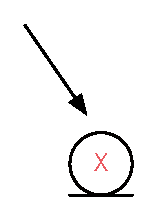
\includegraphics{figs/test1.pdf} 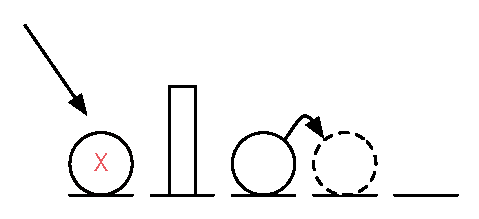
\includegraphics{figs/test2.pdf}
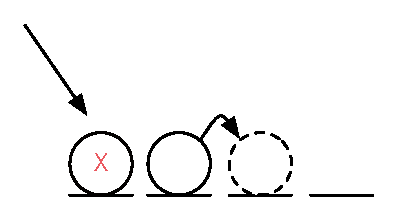
\includegraphics{figs/test3.pdf} 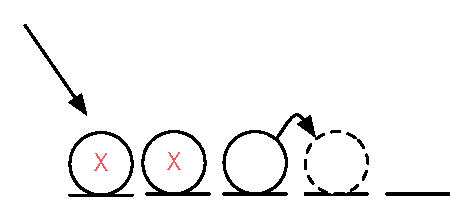
\includegraphics{figs/test4.pdf}
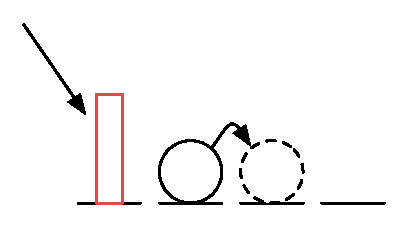
\includegraphics{figs/test5.pdf}

\section{Sample Output:}

When running the pigs:

\begin{verbatim}
Starting pig on port: 10001
Starting pig on port: 10002
Starting pig on port: 10003
Starting pig on port: 10004
Starting pig on port: 10005
Starting pig on port: 10006
Starting pig on port: 10007
Starting pig on port: 10008
Starting pig on port: 10009
Starting pig on port: 10010
\end{verbatim}

When running the game:

\begin{verbatim}
Gathering Pigs...
Looking up on port: 10001
Checking alive: Position(-1)
Looking up on port: 10002
Checking alive: Position(-1)
Looking up on port: 10003
Checking alive: Position(-1)
Looking up on port: 10004
Checking alive: Position(-1)
Looking up on port: 10005
Checking alive: Position(-1)
Looking up on port: 10006
Checking alive: Position(-1)
Looking up on port: 10007
Checking alive: Position(-1)
Looking up on port: 10008
Checking alive: Position(-1)
Looking up on port: 10009
Checking alive: Position(-1)
Looking up on port: 10010
Checking alive: Position(-1)
done gathering.
Can we communicate with the first pig?: Position(-1)
done setting mid positions
done setting end positions

  -----------------------
  |  Initial locations  |
  -----------------------

       |                 |     |                 |        | 
 @  _  |  _  _  @  @  @  |  @  |  @  _  @  @  @  |  @  _  | 
------------------------------------------------------------
Time to target: 589

  -----------------------
  |  Final locations    |
  -----------------------


       |                 |     |                 |        | 
 @  _  |  _  _  @  @  @  |  @  |  @  _  @  @  @  |  @  _  | 
------------------------------------------------------------
                           XXX                                    <- TARGET
\end{verbatim}

\end{document}
